
\section{Experimental Evaluation}
\begin{figure}[htb!]
    \centering
    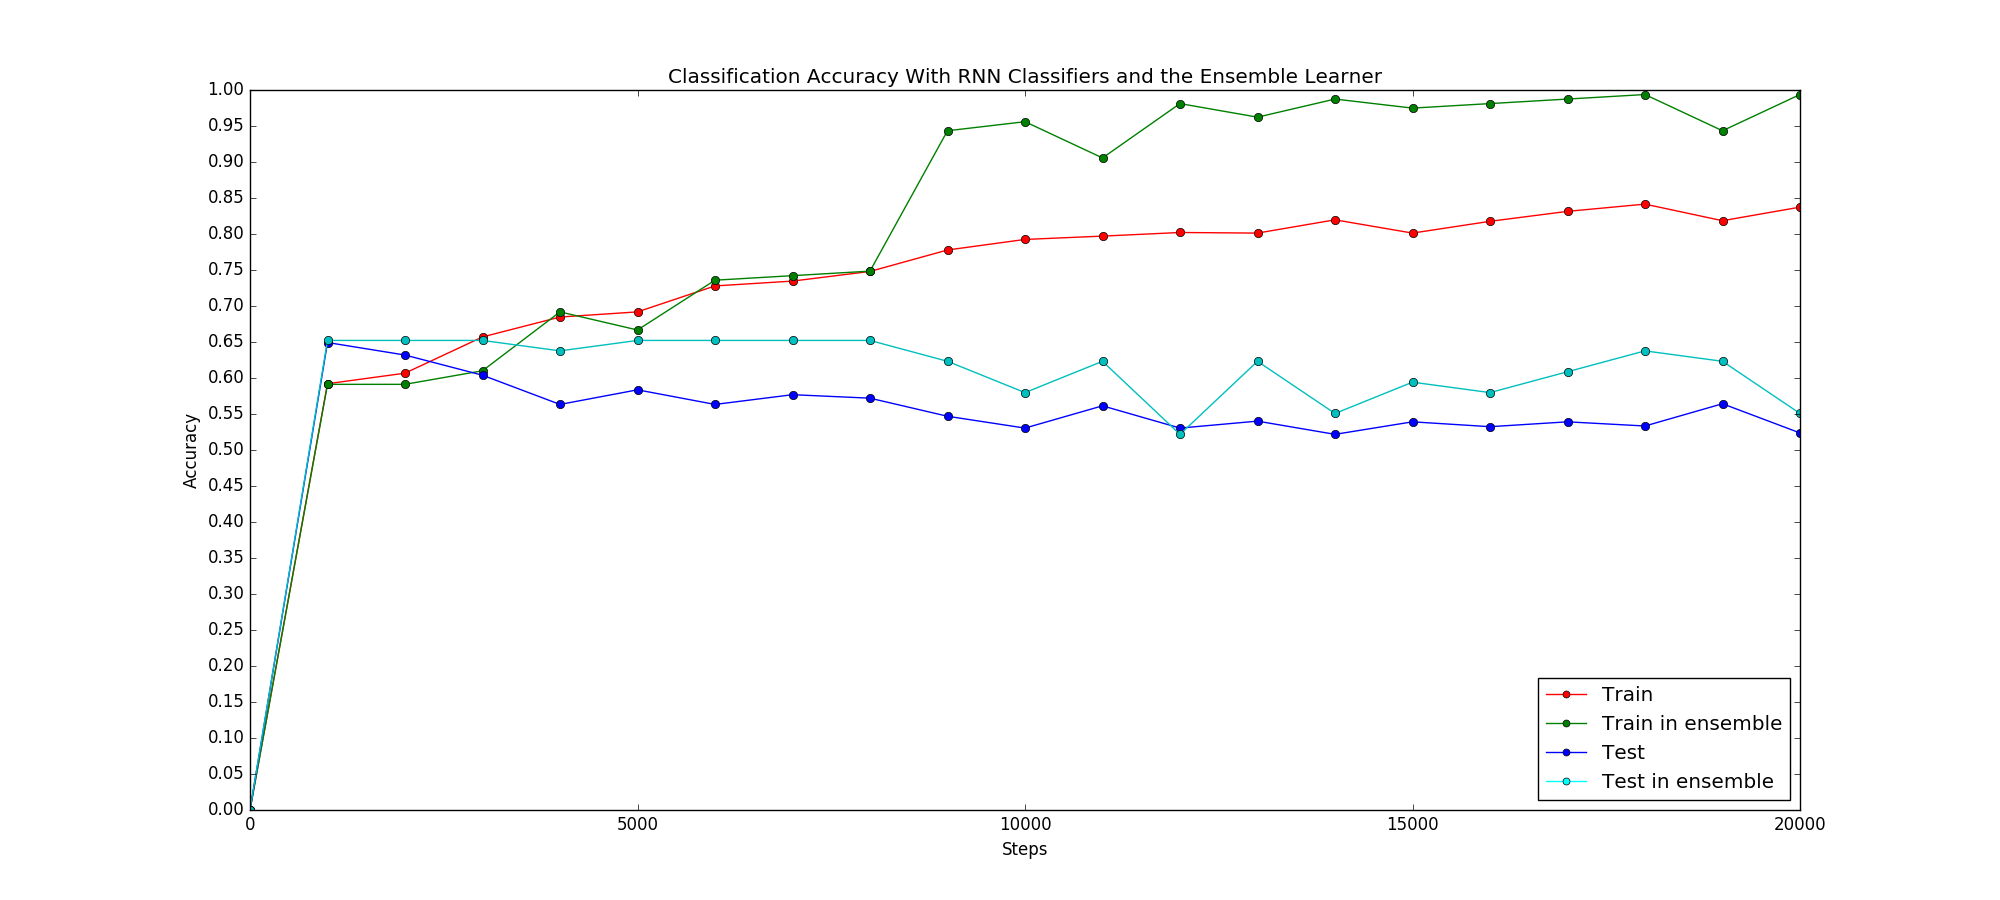
\includegraphics[width=0.9\textwidth]{typical_case.png}
    \caption{A typical training case.}
    \label{fig:awesome_image}
\end{figure}
\FloatBarrier
Figure 4 is a typical accuracy plot when training the RNN model. In this experiment, the length of the time series is set as 135, which is splitted into 15 segments with each sub-series length 9. The vector size of each time point in the time series (i.e. the output dimension of the DAE) is 5. Each batch of 15 examples is fed into the Adadelta optimizer with its initial learning rate 1. We choose tanh activation function, which apparently accelerate the learning in the series of experiments. Both accuracy for sub-series and ensemble accuracy are reported in the graph. Compared to mini-batch Gradient Descent Optimizer (which is not shown here), Adadelta optimizer shows better converge property for this classification task.  After 200,000 steps (about 58 epoches), the ensemble training accuracy arrives 100\% although the training accuracy is just beyond 80\%. In the steps before 5000, there is a obvious platform for the training accuracies, which might be brought by neuron saturation. The testing performance reaches its maximum value  (around 65\%) very quickly in the training. However, it begins to drop since training accuracy begin a relative rapid increase period. This implies that early stop technique need to be employed in this classification task although dropout technique already makes significant improvements in preventing overfitting. The ensemble accuracies for the testing data are always higher than their corresponding accuracies without ensemble. Since data fed into the high-level classifiers are not dependent, these accuracies are much lower than what are expected.



\begin{figure}[!htbp]
    \centering
    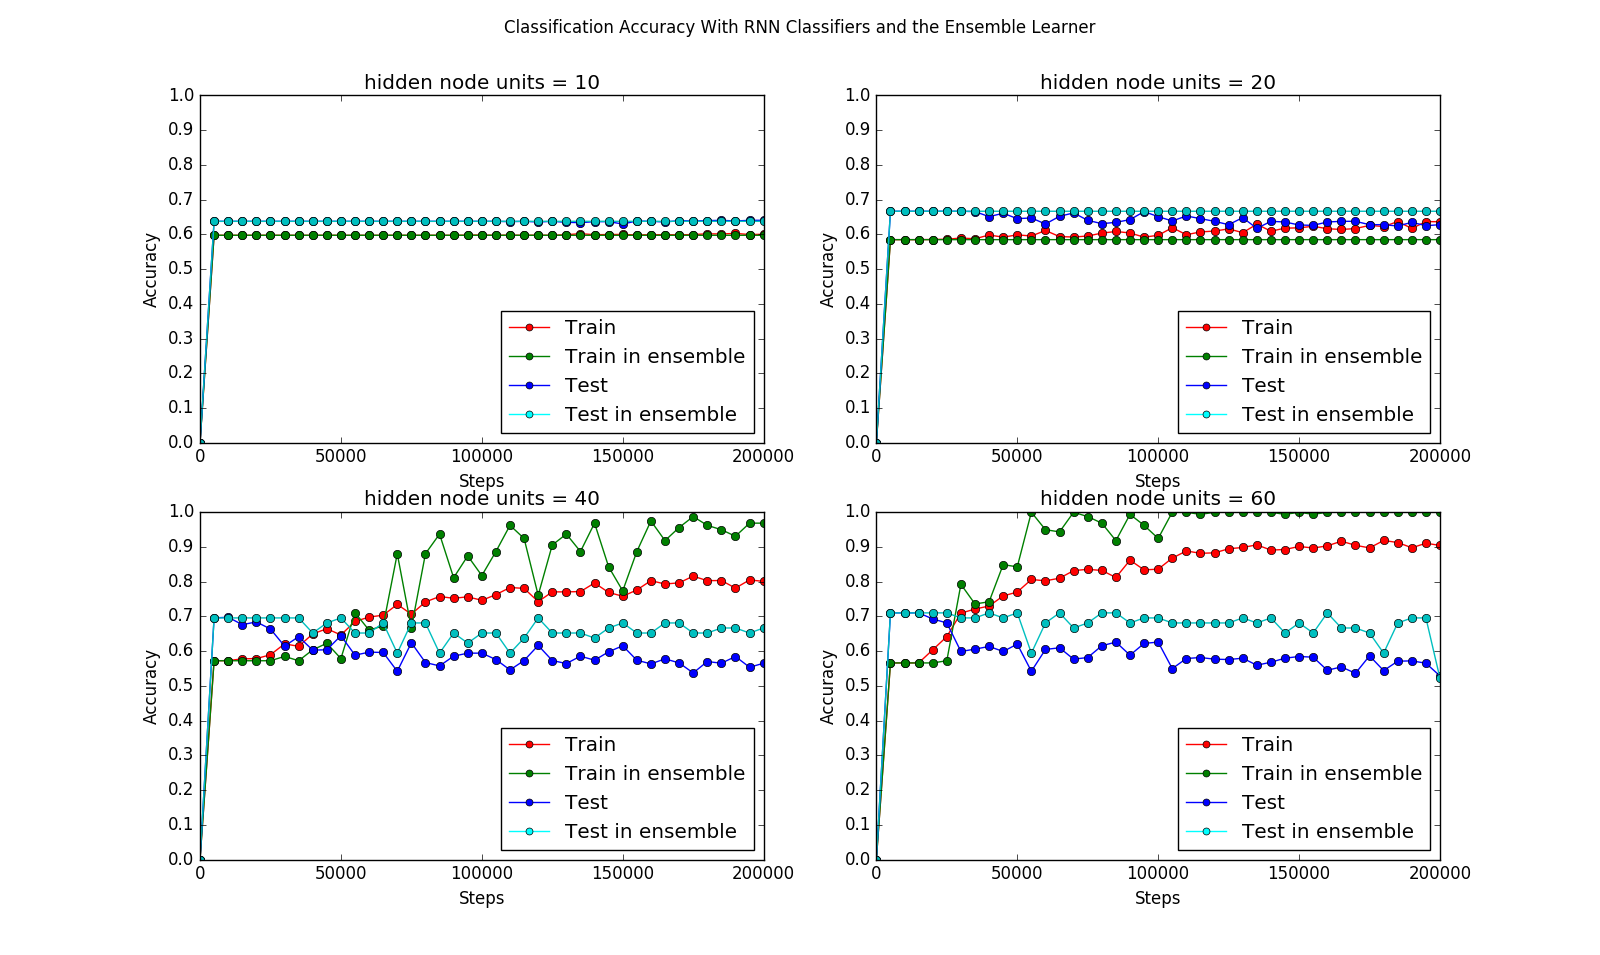
\includegraphics[width=0.9\textwidth]{state_size.png}
    \caption{The influence of hidden node units number on accuracy.}
    \label{fig:awesome_image}
\end{figure}

\begin{figure}[!htbp]
    \centering
    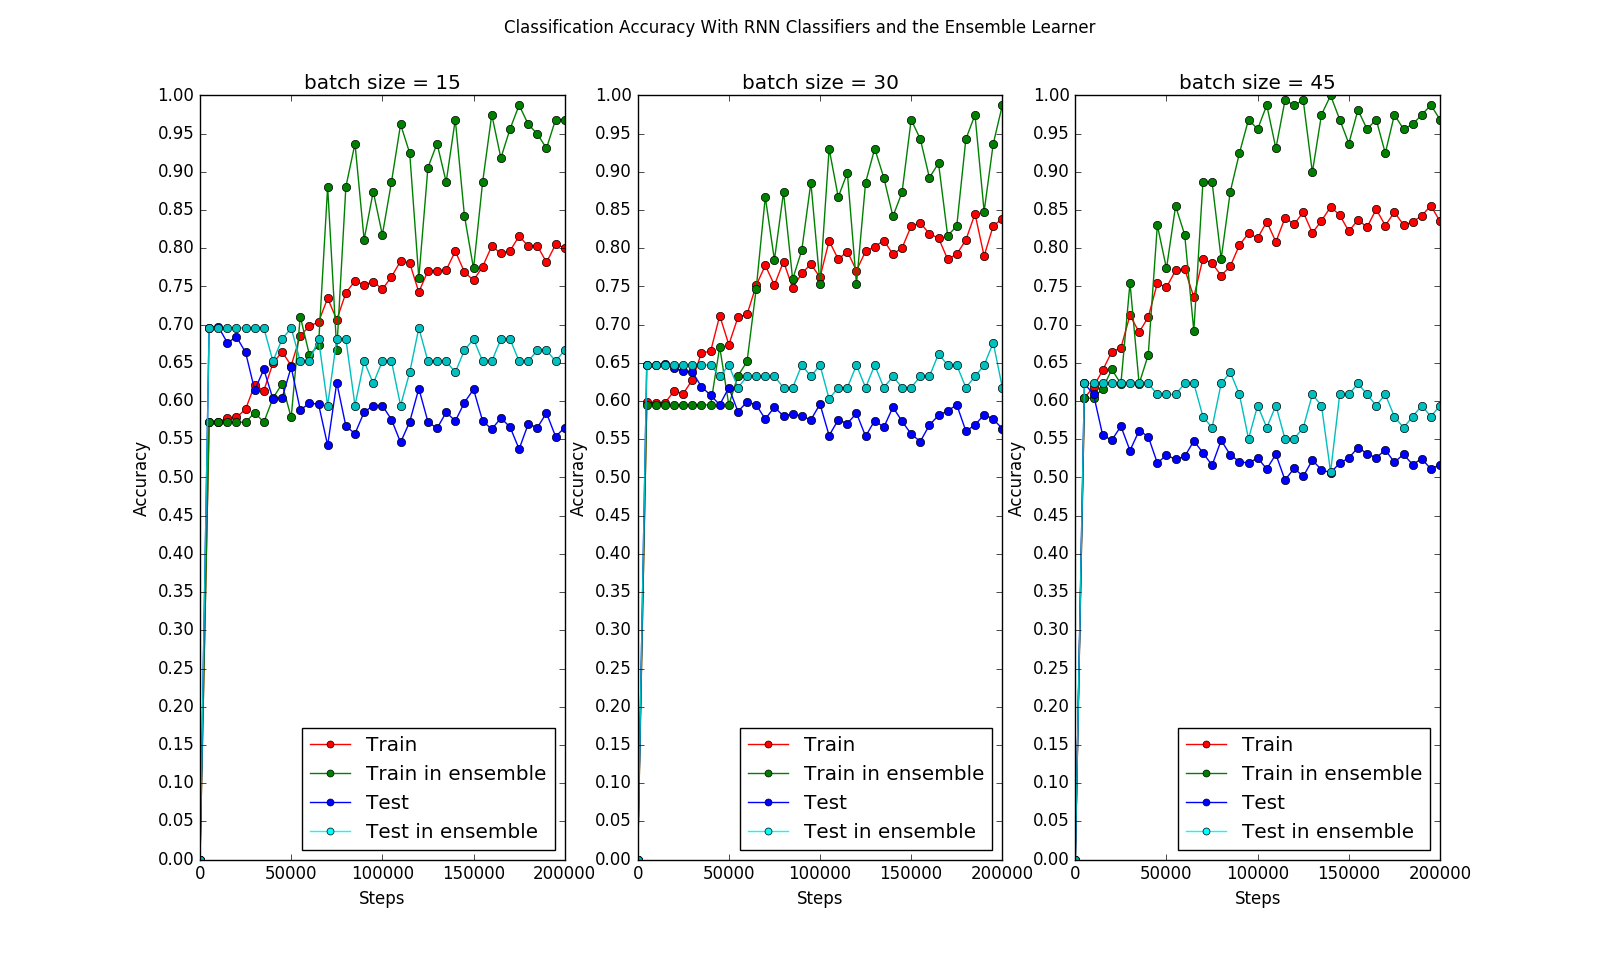
\includegraphics[width=0.9\textwidth]{batch_size.png}
    \caption{The influence of batch size on accuracy.}
    \label{fig:awesome_image}
\end{figure}

It is proved by the experiments that number of hidden note units have substantial influence on the final testing accuracy, which can be indicated Figure 5. In this graph, model with 4 different hidden node configuration is plotted. It can be concluded that the learning speed raises with the increase size of hidden units. Even in the 10 hidden node units case, no obvious improvements can be identified between training steps. In terms of testing accuracy, the 60 units case does not have essential enhancement comparing to the 40 units. 

Figure 6 shows the influence of batch size on the accuracy. All the hyper-parameter settings but the batch-size are the same, which shows that relatively low batch size setting can lead to better testing accuracies.



